\section{Μοντελοποίηση Κλάσεων}
\label{sec:class_modeling}

Η οργάνωση του κώδικα έγινε με την μορφή κλάσεων στη γλώσσα Python ενώ όπως έχει αναφερθεί παραπάνω για την γραφική διεπαφή χρησιμοποιήθηκε η βιβλιοθήκη Kivy. Στο παρόν κεφάλαιο θα παρουσιαστούν όλες οι κλάσεις που υλοποιήθηκαν για το λογισμικό του καθρέφτη μαζί με τις μεταβλητές και μεθόδους που ανήκουν σε κάθε κλάση, ενώ θα γίνει και μια περιγραφή του κάθε μέλους. Με τέτοιου είδους διαγράμματα είναι εφικτό να μοντελοποιηθεί το λογισμικό σε ανώτερο επίπεδο και χωρίς να χρειαστεί να κοιτάξουμε άμεσα τον κώδικα \cite{ClassDiagrams}. Η περιγραφή των κλάσεων θα γίνει στην γλώσσα UML\footnote{\href{https://en.wikipedia.org/wiki/Unified\_Modeling\_Language}{https://en.wikipedia.org/wiki/Unified\_Modeling\_Language}} κατά την οποία, όπως φαίνεται στο Σχήμα \ref{fig:class_diagram_example}, μια κλάση αναπαριστάται από 3 μέρη, το όνομά της, τα χαρακτηριστικά (μεταβλητές) της και τέλος οι μέθοδοί της.

\begin{figure}[h]
    \centering
    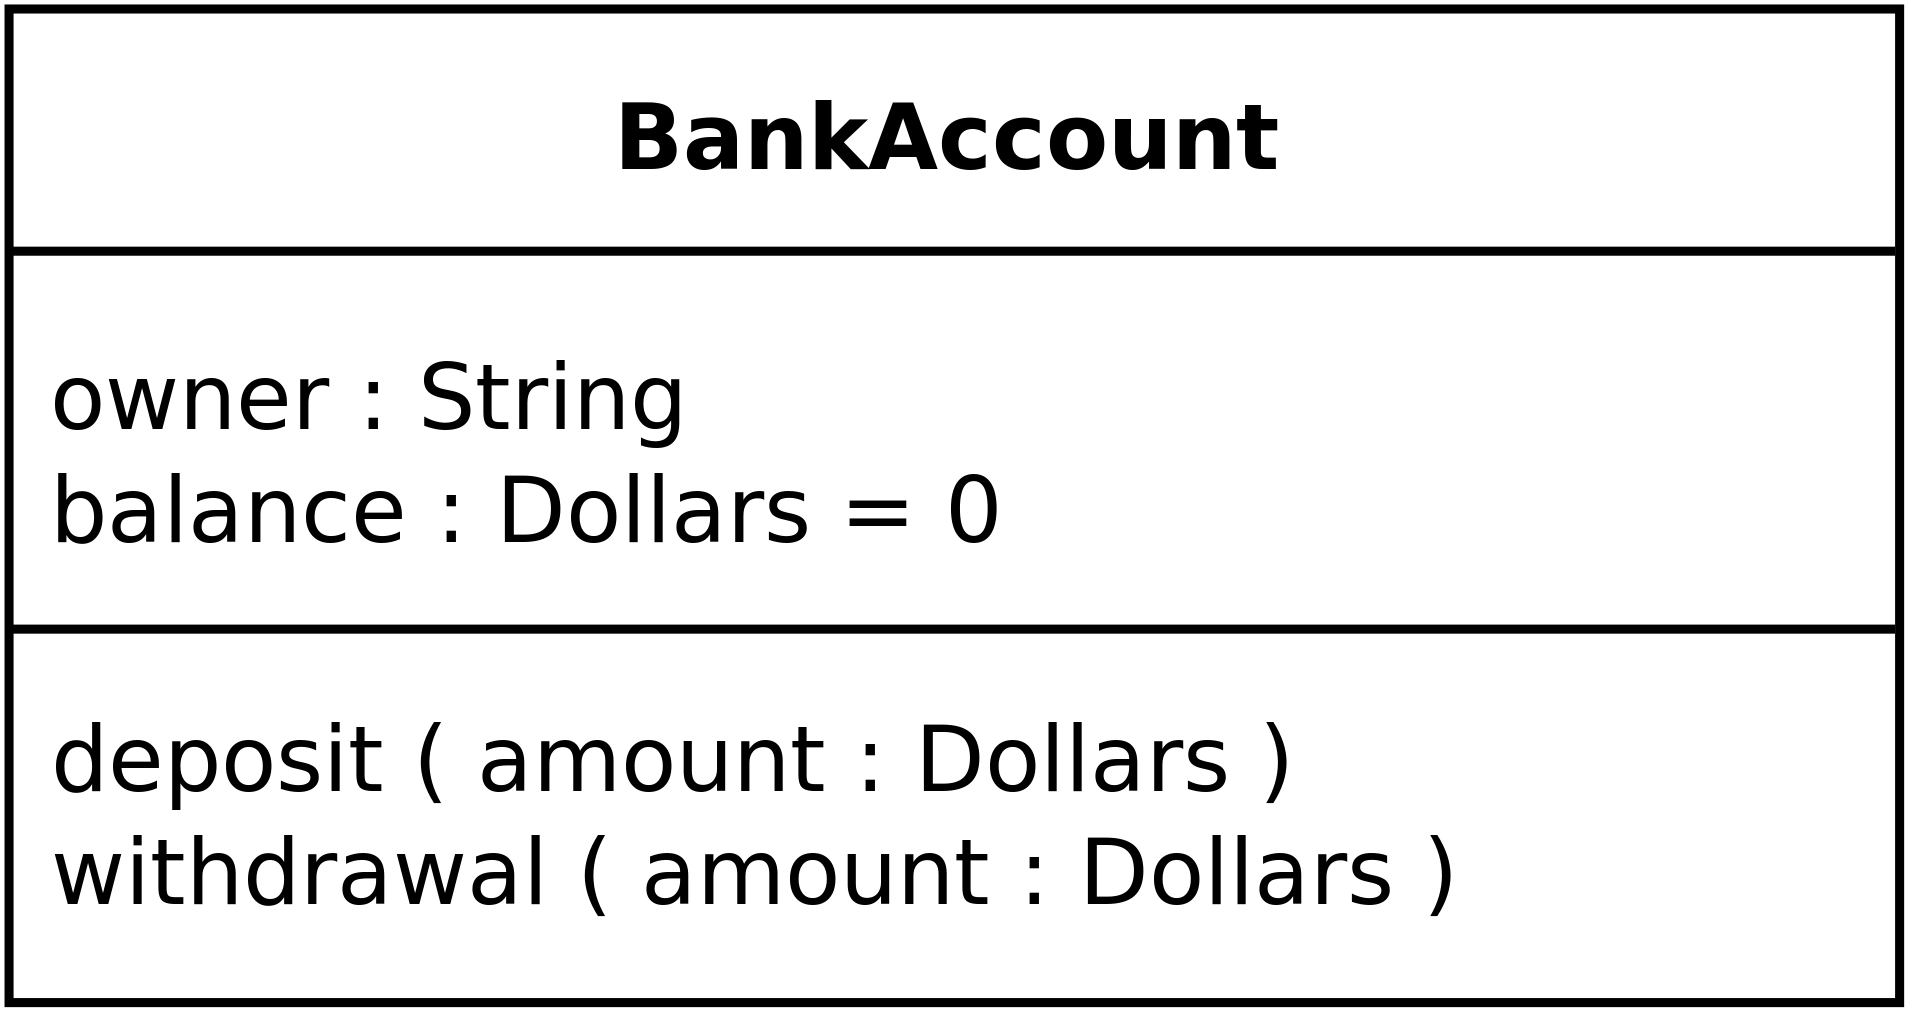
\includegraphics[scale=0.1]{images/chapter4/uml_diagrams/class_diagram_example.png}
    \caption{Παράδειγμα αναπαράστασης κλάσης στη UML}
    \label{fig:class_diagram_example}
\end{figure}

\subsection{SmartMirrorApp}

\begin{figure}[h]
    \centering
    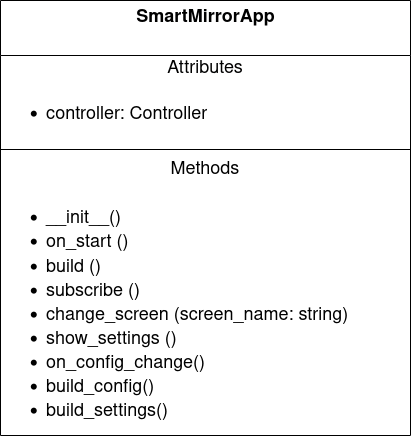
\includegraphics[scale=0.7]{images/chapter4/uml_diagrams/SmartMirrorApp.png}
    \caption{UML της κλάσης SmartMirrorApp}
    \label{fig:smartmirrorapp}
\end{figure}
\noindent\textbf{Περιγραφή Κλάσης}

Η κλάση αυτή κληρονομεί από την κλάση \href{https://kivy.org/doc/stable/api-kivy.app.html\#kivy.app.App}{\texttt{kivy.app.App}} η οποία είναι η βασική κλάση για την δημιουργία μιας Kivy εφαρμογής. Μέσως αυτής της κλάσης ελέγχουμε την γραφική εφαρμογή και όταν όλα είναι έτοιμα ξεκινάμε τον κύκλο ζωής της εφαρμογής καλώντας την μέθοδο \texttt{SmartMirrorApp().run()}.

\noindent\textbf{Χαρακτηριστικά Κλάσης}
\begin{itemize}
    \item \texttt{controller}: Αντικείμενο τύπου Controller για την ενεργοποίηση του thread ελέγχου.
\end{itemize}

\noindent\textbf{Μέθοδοι Κλάσης}
\begin{itemize}
    \item \texttt{\_\_init\_\_()}: Συνάρτηση δόμησης της κλάσης η οποία καλή την συνάρτηση δόμησης της κλάσης \texttt{kivy.app.App} μέσω του \texttt{super()} και αρχικοποιεί τη μεταβλητή \texttt{controller} να είναι \texttt{None}.
    
    \item \texttt{on\_start()}: Ειδική μέθοδος της κλάσης \texttt{kivy.app.App} που εκτελείται λίγο πριν την εκκίνηση της εφαρμογής (αμέσως μετά την συνάρτηση \texttt{build()}. Δημιουργεί το αντικείμενο \texttt{Controller} και ξεκινάει το thread ελέγχου.
    
    \item \texttt{build()}: Ειδική μέθοδος της κλάσης \texttt{kivy.app.App} η οποία αρχικοποιεί την εφαρμογή και εκτελείται μόνο μία φορά. Φορτώνει όλες τις εγκατεστημένες εφαρμογές και επιστρέφει το βασικό Widget (ένα στιγμιότυπο της κλάσης MainPage η οποία θα εξηγηθεί παρακάτω).
    
    \item \texttt{subscribe()}: Μέθοδος η οποία επιστρέφει ένα Python dictionary όπου γίνεται μια αντιστοίχηση ενός intent σε μια συνάρτηση. Η μέθοδος αυτή χρησιμοποιείται προκειμένου να μπορεί να εκτελεστεί η σωστή συνάρτηση όταν γίνει αναγνώριση της πρόθεσης της εντολής του χρήστη από το Wit.ai. 
    
    \item \texttt{change\_screen(screen\_name: string)}: Συνάρτηση που χρησιμοποείται για να γίνει αλλαγή Screen δηλαδή να φορτώσει μια άλλη εφαρμογή με όνομα \texttt{screen\_name}.
    
    \item \texttt{show\_settings()}: Μέθοδος η οποία καλεί την συνάρτηση \texttt{open\_settings} της κλάσης \texttt{kivy.app.App} για να ανοίξει το μενού ρυθμίσεων της εφαρμογής.
    
    \item \texttt{on\_config\_change()}: Ειδική μέθοδος της κλάσης \texttt{kivy.app.App} η οποία εκτελείται όταν γίνει κάποια αλλαγή ρύθμισης. Για κάθε ένα από τα εγκατεστημένα Widgets ανανεώνει τις ρυθμίσεις τους.
    
    \item \texttt{build\_config()}: Ειδική μέθοδος της κλάσης \texttt{kivy.app.App} η οποία
    εκτελείται πριν την αρχικοποίηση της εφαρμογής και δημιουργεί default ρυθμίσεις για κάθε ένα από τα εγκατεστημένα Widgets.
    
    \item \texttt{build\_settings()}: Ειδική μέθοδος της κλάσης \texttt{kivy.app.App} η οποία εκτελείται όταν θέλουμε να δείξουμε τις ρυθμίσεις της εφαρμογής. Διαβάζει από κάθε εγκατεστημένο Widget τις ρυθμίσεις τους (οι οποίες βρίσκονται σε ένα αρχείο "settings.json" και τις προσθέτει στο μενού ρυθμίσεων.
    
\end{itemize}

\newpage
\subsection{MainPage}

\begin{figure}[h]
    \centering
    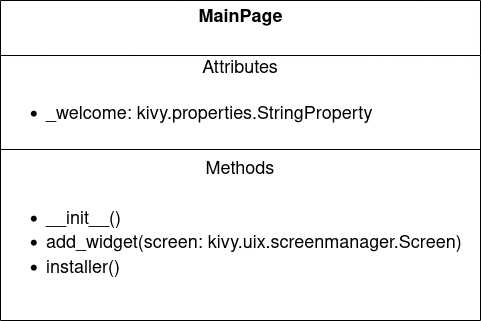
\includegraphics[scale=0.7]{images/chapter4/uml_diagrams/MainPage.png}
    \caption{UML της κλάσης MainPage}
    \label{fig:mainpage}
\end{figure}

\noindent\textbf{Περιγραφή Κλάσης}

Η κλάση αυτή κληρονομεί από την κλάση \href{https://kivy.org/doc/stable/api-kivy.uix.screenmanager.html\#kivy.uix.screenmanager.ScreenManager}{ScreenManager} που περιέχεται στο πακέτο \texttt{kivy.uix.screenmanager}. Η κλάση αυτή είναι το πρωτεύον Widget που επιστρέφει η εφαρμογή και κάτω από αυτήν μπαίνουν όλες οι εφαρμογές που εγκαθιστά ο χρήστης (σαν καινούργια Screens).

\noindent\textbf{Χαρακτηριστικά Κλάσης}
\begin{itemize}
    \item \texttt{\_welcome}: Μεταβλητή που χρησιμοποιείται για να αποθηκεύσει ένα μήνυμα που καλωσορίζει τον χρήστη.
\end{itemize}

\noindent\textbf{Μέθοδοι Κλάσης}
\begin{itemize}
    \item \texttt{\_\_init\_\_()}: Η συνάρτηση δόμησης της κλάσης η οποία καλή την συνάρτηση δόμησης της κλάσης \texttt{kivy.uix.screenmanager.ScreenManager} μέσω του \texttt{super} και αρχικοποιεί τη μεταβλητή \texttt{\_welcome} να πάρει μία τυχαία επιλογή από μια λίστα μηνυμάτων. Τέλος καλεί την εσωτερική συνάρτηση \texttt{installer} προκειμένου να εγκαταστήσει όλες τις εφαρμογές που βρίσκονται στον φάκελο \texttt{/widgets} σαν ξεχωριστά Screens.
    
    \item \texttt{add\_widget(screen: kivy.uix.screenmanager.Screen)}: Ειδική συνάρτηση της κλάσης \texttt{kivy.uix.screenmanager.ScreenManager} η οποία προσθέτει ένα καινούργιο Widget στα παιδιά του τρέχοντος Widget. Στην υπερφορτωμένη της έκδοση, επιτρέπεται η πρόσθεση μόνο ενός Widget τύπου \texttt{kivy.uix.screenmanager.Screen} για περισσότερη ασφάλεια.
    
    \item \texttt{installer()}: Συνάρτηση η οποία για κάθε ένα από τα παιδιά της \texttt{MainPage} καλεί την συνάρτηση \texttt{install} την οποία πρέπει να ορίσουν οι εξωτερικές εφαρμογές προκειμένου να μπορούν να εγκατασταθούν από τον καθρέφτη.
\end{itemize}

\subsection{Controller}
\begin{figure}[h!]
    \centering
    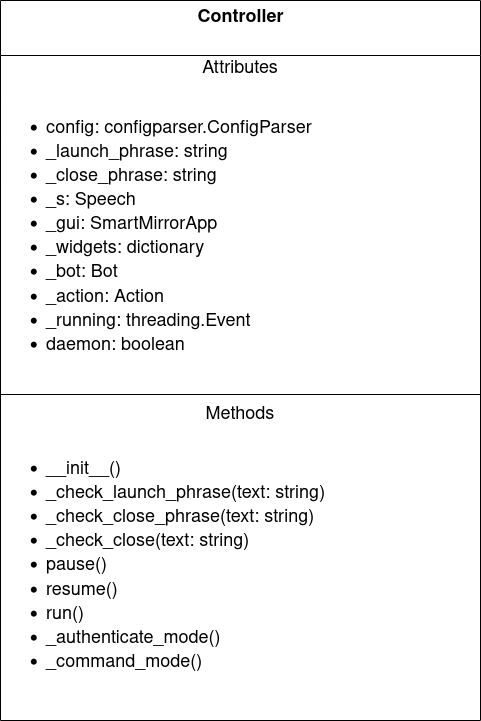
\includegraphics[scale=0.7]{images/chapter4/uml_diagrams/Controller.png}
    \caption{UML της κλάσης Controller}
    \label{fig:controller}
\end{figure}
\noindent\textbf{Περιγραφή Κλάσης}

Η κλάση αυτή κληρονομεί από την κλάση \href{https://docs.python.org/3/library/threading.html\#threading.Thread}{threading.Thread}. O controller είναι ένα ανεξάρτητο thread από το main thread στο οποίο τρέχει η γραφική εφαρμογή και είναι υπεύθυνος για τον έλεγχο των λειτουργιών του συστήματος. Μέσα από αυτήν την κλάση ελέγχεται η ροή του προγράμματος, επιλέγονται οι ενέργειες που θα εκτελέσει ο καθρέφτης και ανανεώνεται το γραφικό περιβάλλον με βάση τις εντολές του χρήστη.

\noindent\textbf{Χαρακτηριστικά Κλάσης}
\begin{itemize}
    \item \texttt{config}: Αντικείμενο τύπου \texttt{configparser.ConfigParser} για την ανάγνωση ρυθμίσεων.
    \item \texttt{\_launch\_phrase}: Μεταβλητή για την αποθήκευση της φράσης ενεργοποίησης του καθρέφτη.
    \item \texttt{\_close\_phrase}: Μεταβλητή για την αποθήκευση της φράσης απενεργοποίησησς του καθρέφτη.
    \item \texttt{\_s}: Αντικείμενο τύπου \texttt{Speech} το οποίο χρησιμοποιείται για την αναγνώριση της φωνής του χρήστη.
    \item \texttt{\_gui}: Αντικείμενο τύπου \texttt{SmartMirrorApp} το οποίο χρησιμοποιείται για να γίνεται αλληλεπίδραση μεταξύ του Controller και του γραφικού περιβάλλοντος.
    \item \texttt{\_widgets}: Dictionary το οποίο αποθηκεύει όλα τα Widgets του γραφικού περιβάλοντος με τα ids τους ως κλειδιά.
    \item \texttt{\_bot}: Αντικείμενο τύπου \texttt{Bot} το οποίο χρησιμοποιείται για την αλληλεπίδραση με το Wit.ai.
    \item \texttt{\_action}: Αντικείμενο τύπου \texttt{Action} το οποίο χρησιμοποιείται ως βοηθημα για την εκτέλεση της εντολής του χρήστη.
    \item \texttt{\_running}: Μεταβλητή τύπου \texttt{threading.Event} η οποία χρησιμοποιείται για τον έλεγχο του Thread του Controller.
    \item \texttt{daemon}: Μεταβλητή που καθορίζει αν το Thread θα εκτελεστεί στο προσκήνιο ή στο παρασκήνιο.
\end{itemize}
\noindent\textbf{Μέθοδοι Κλάσης}
\begin{itemize}
    \item \texttt{\_\_init\_\_()}: Η συνάρτηση δόμησης της κλάσης διαβάζει από τις ρυθμίσεις τις φράσεις ενεργοποίησης/απενεργοποίησης, αρχικοποιεί τα αντικείμενα των βοηθητικών κλάσεων που θα χρησιμοποιηθούν για τον έλεγχο του καθρέφτη και τέλος ξεκινάει ένα Thread στο παρασκήνιο στο οποίο θα γίνεται ο λογικός έλεγχος της ροής του προγράμματος.
    \item \texttt{\_check\_launch\_phrase(text: String)}: Βοηθητική συνάρτηση όπου επιστρέφει True αν η μεταβλητή \texttt{text} ταυτίζεται με την φράση έναρξης και False σε αντίθετη περίπτωση.
    \item \texttt{\_check\_close\_phrase(text: String)}: Βοηθητική συνάρτηση όπου επιστρέφει True αν η μεταβλητή \texttt{text} ταυτίζεται με την φράση απενεργοποίησης και False σε αντίθετη περίπτωση.
    \item \texttt{\_check\_close(text: String)}: Βοηθητική συνάρτηση που ελέγχει εαν η μεταβλητή \texttt{text} είναι ίση με \texttt{"quit"} ή \texttt{"exit"} προκειμένου να διακόψει τη λειτουργία του καθρέφτη.
    \item \texttt{pause()}: Βοηθητική συνάρτηση η οποία σταματάει το Thread του Controller.
    \item \texttt{resume()}: Βοηθητική συνάρτηση η οποία ενεργοποιεί το Thread του Controller.
    \item \texttt{run()}: H συνάρτηση αυτή ενεργοποιεί το Thread του Controller και καλεί τις συναρτήσεις \texttt{\_authenticate\_mode()} και \texttt{\_command\_mode()} η οποίες ελέγχουν την κατάσταση του καθρέφτη.
    \item \texttt{\_authenticate\_mode()}: Στη συγκεκριμένη κατάσταση ο καθρέφτης είναι αδρανής και περιμένει να ακούσει την φράση ενεργοποίησης προκειμένου να δώσει πρόσβαση στον χρήστη και να ακολουθεί τις εντολές του. Με αυτόν τον τρόπο ο καθρέφτης θα ακούει τις εντολές του χρήστη μόνο όταν αυτός το θέλει.
    \item \texttt{\_command\_mode()}: Στη συγκεκριμένη κατάσταση γίνεται ο έλεγχος της ροής του καθρέφτη όπου γίνεται επαναληπτικά η ακοή της εντολής του χρήστη, η αλληλεπίδραση με το Wit.ai για την αναγνώριση της πρόθεσης του χρήστη και η εκτέλεση της εντολής αν αυτή είναι αποδεκτή. Η επανάληψη συνεχίζεται έως ότου ο χρήστης πει την φράση απενεργοποίησης ή μία εκ των εντολών "quit" και "exit" οι οποίες απενεργοποιούν τον καθρέφτη.
\end{itemize}
\newpage
\subsection{Speech}
\begin{figure}[h]
    \centering
    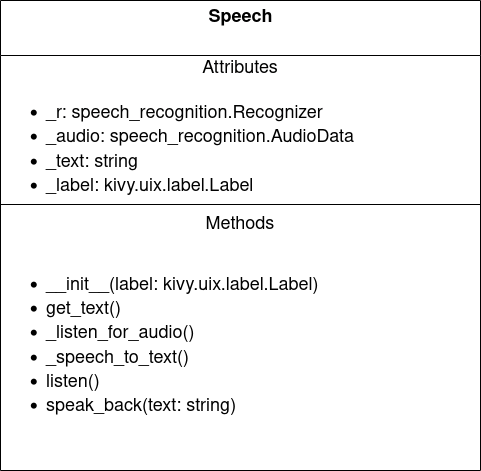
\includegraphics[scale=0.7]{images/chapter4/uml_diagrams/Speech.png}
    \caption{UML της κλάσης Speech}
    \label{fig:speech}
\end{figure}
\noindent\textbf{Περιγραφή Κλάσης}

Η κλάση αυτή υλοποιεί όλες τις μεθόδους και την διεπαφή για την ανάγνωση και ομιλία ήχου. Μέσω αυτής της κλάσης ο καθρέφτης μπορεί να ακούει τον χρήστη από το μικρόφωνο ανά τακτά διαστήματα και να μετατρέπει τις εντολές του σε κείμενο το οποίο θα χρησιμοποιηθεί αργότερα για την αναγνώριση της πρόθεσης. Τέλος, μέσω αυτής της κλάσης ο καθρέφτης δύναται να μιλήσει στον χρήστη, λέγοντάς του αποτελέσματα ενεργειών ή πληροφορίες.

\noindent\textbf{Χαρακτηριστικά Κλάσης}
\begin{itemize}
    \item \texttt{\_r}: Αντικείμενο τύπου \texttt{speech\_recognition.Recognizer} μέσω του οποίο γίνεται η ανάγνωση της φωνής και η αναγνώρισή της σε κείμενο.
    \item \texttt{\_audio}: Αντικείμενο τύπου \texttt{speech\_recognition.AudioData} το οποίο αποθηκεύει τα δεδομένα του ήχου τα οποία χρησιμοποιούνται για την αναγνώριση και μετατροπή σε κείμενο.
    \item \texttt{\_text}: Μεταβλητή στην οποία αποθηκεύεται σε γραπτή μορφή η εντολή του χρήστη μετά την αναγνώριση.
    \item \texttt{\_label}: Αντικείμενο τύπου \texttt{kivy.uix.label.Label} το οποίο χρησιμοποιείται προκειμένου να εμφανίζεται στην οθόνη του καθρέφτη πότε το σύστημα ακούει εντολές από τον χρήστη.
\end{itemize}
\noindent\textbf{Μέθοδοι Κλάσης}
\begin{itemize}
    \item \texttt{\_\_init\_\_(kivy.uix.label.Label)}: Συνάρτηση δόμησης της κλάσης η οποία αρχικοποιεί τις μεταβλητές που χρησιμποιεί η κλάση και δέχεται ως είσοδο το Label στο οποίο θα υποδηλώνεται πότε ο καθρέφτης ακούει για εντολές.
    \item \texttt{get\_text()}: Βοηθητική συνάρτηση η οποία επιστρέφει την τιμή της μεταβλητής \texttt{\_text}.
    \item \texttt{\_listen\_for\_audio()}: Βοηθητική συνάρτηση η οποία ακούει από το μικρόφωνο τις εντολές του χρήστη. Η λειτουργία ανάγνωσης του ήχου από το μικρόφωνο του συστήματος γίνεται με την αρχικοποίηση ενός αντικειμένου τύπου \texttt{speech\_recognition.Microphone}. Τα δεδομένα ήχου αποθηκεύονται στο αντικείμενο \texttt{\_audio} ενώ γίνεται και εγγραφή στο Label του καθρέφτη για την ενημέρωση του χρήστη ότι το σύστημα περιμένει εντολή.
    \item \texttt{\_speech\_to\_text()}: Συνάρτηση που καλεί την μέθοδο \texttt{recognize\_google()} του αντικειμένου \texttt{\_r} η οποία αλληλεπιδρά με το API της Google για την μετατροπή των δεδομένων ήχου σε κείμενο. Σε περίπτωση που δεν γίνεται αναγνώριση το κείμενο τίθεται κενό.
    \item \texttt{listen()}: Συνάρτηση η οποία καλείται από τον Controller και καλεί τις 2 συναρτήσεις για ανάγνωση του ήχου και μετατροπή σε κείμενο.
    \item \texttt{speak\_back(text: string)}: Συνάρτηση η οποία καλείται εξωτερικά για την ομιλία του καθρέφτη προς τον χρήστη. Μέσω της βιβλιοθήκης gTTS μετατρέπεται το κειμενο εισόδου σε ομιλία, αποθηκεύεται ως ένα προσωρινό αρχείο .mp3 και αναπαράγεται μέσω της βιβλιοθήκης pydub. Τέλος, το προσωρινό αρχείο διαγράφεται.
\end{itemize}
\newpage
\subsection{Bot}
\begin{figure}[h]
    \centering
    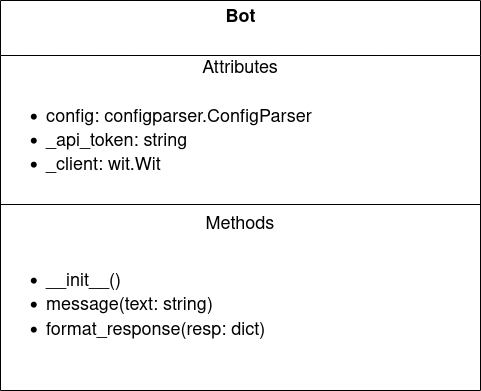
\includegraphics[scale=0.7]{images/chapter4/uml_diagrams/Bot.png}
    \caption{UML της κλάσης Bot}
    \label{fig:bot}
\end{figure}
\noindent\textbf{Περιγραφή Κλάσης}

Η κλάση αυτή αποτελεί την διεπαφή για την αλληλεπίδραση με το Wit.ai και την εξαγωγή της πρόθεσης της εντολής του χρήστη αλλά και των οντοτήτων οι οποίες θα δοθούν ως ορίσματα κατά την εκτέλεση των εντολών.

\noindent\textbf{Χαρακτηριστικά Κλάσης}
\begin{itemize}
    \item \texttt{config}: Αντικείμενο τύπου \texttt{configparser.ConfigParser} για την ανάγνωση ρυθμίσεων.
    \item \texttt{\_api\_token}: Μεταβλητή η οποία αποθηκεύει το api\_key που χρησιμοποιείται για να αποκτήσει η εφαρμογή πρόσβαση στο Wit.ai.
    \item \texttt{\_client}: Αντικείμενο τύπου \texttt{wit.Wit} μέσω του οποίου θα γίνεται η αλληλεπίδραση με το Wit.ai.
\end{itemize}
\noindent\textbf{Μέθοδοι Κλάσης}
\begin{itemize}
    \item \texttt{\_\_init\_\_()}: Συνάρτηση δόμησης της κλάσης η οποία διαβάζει το κλειδί από τις ρυθμίσεις και αρχικοποιεί ένα αντικείμενο τύπου \texttt{wit.Wit}.
    \item \texttt{message(text: string)}: Η συνάρτηση που καλείται από τον Controller, στέλνει την εντολή σε μορφή κειμένου στο Wit.ai και επιστρέφει την πρόθεση και τις οντότητες που εξάγονται. Σε περίπτωση που δεν αναγνωριστεί η εντολή γίνεται κατάλληλος έλεγχος σφάλματος.
    \item \texttt{format\_response(resp: dict)}: Βοηθητική συνάρτηση η οποία δέχεται ως είσοδο το αποτέλεσμα του Wit.ai και μορφοποιεί την πρόθεση και τις οντότητες στην επιθυμητή μορφή ενός dictionary.
\end{itemize}

\subsection{Action}
\begin{figure}[h]
    \centering
    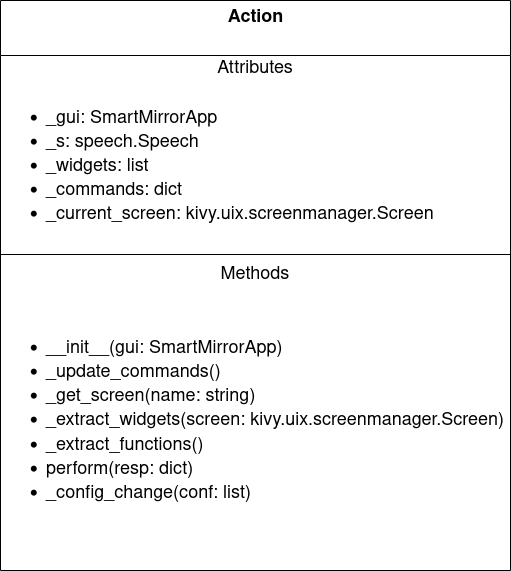
\includegraphics[scale=0.7]{images/chapter4/uml_diagrams/Action.png}
    \caption{UML της κλάσης Action}
    \label{fig:action}
\end{figure}
\noindent\textbf{Περιγραφή Κλάσης}

Η κλάση αυτή αποτελεί την διεπαφή για την εκτέλεση των εντολών του χρήστη και είναι στην ουσία μια επέκταση του Controller. Μέσω της συγκεκριμένης κλάσης, γίνεται η μετατροπή της πρόθεσης που παίρνει το σύστημα από το Wit.ai σε εκτέλεση της κατάλληλης πράξης που υποδηλώνεται από την πρόθεση (αν αυτή υπάρχει και είναι προσβάσιμη).
\newpage
\noindent\textbf{Χαρακτηριστικά Κλάσης}
\begin{itemize}
    \item \texttt{\_gui}: Αντικείμενο τύπου \texttt{SmartMirrorApp} το οποίο χρησιμοποιείται για να γίνεται αλληλεπίδραση μεταξύ του Controller και του γραφικού περιβάλλοντος.
    \item \texttt{\_s}: Αντικείμενο τύπου \texttt{Speech} το οποίο χρησιμοποιείται για την ομιλία του καθρέφτη προς τον χρήστη.
    \item \texttt{\_widgets}: Μία λίστα που αποθηκεύει όλα τα Widgets που βρίσκονται στην τωρινή οθόνη και το αντικείμενο \_gui.
    \item \texttt{\_commands}: Ένα dictionary που αποθηκεύει τις δυνατές εντολές που εξάγει κάθε Widget ως κλειδιά μαζί με τις αντίστοιχες συναρτήσεις που θα κληθούν για την κάθε εντολή ως τιμές.
    \item \texttt{\_current\_screen}: Αντικείμενο τύπου kivy.uix.screenmanager.Screen το οποίο έχει την τιμή της οθόνης στην οποία βρίσκεται κάθε στιγμή ο καθρέφτης.
\end{itemize}
\noindent\textbf{Μέθοδοι Κλάσης}
\begin{itemize}
    \item \texttt{\_\_init\_\_(gui: SmartMirrorApp)}:
\end{itemize}